% intro should describe and justify this cahpter
% 
\graphicspath{{chapters/3.Chapter_1/figures/}}


\begin{savequote}[75mm]
    Taxonomy is described sometimes as a science and sometimes as an art, but really it's a battleground
    \qauthor{- Bill Bryson: \textit{A Short History of Nearly Everything}}
\end{savequote}

\chapter{Endosymbiont diversity}\label{chap:endo_diversity}

\section{Introduction}

\subsection{Endosymbiont taxonomy and clonality}

Over 50 strains of green algal photobionts have been identified in 
\textit{Paramecium bursaria} species \citep{Hoshina2010,Hoshina2004,Hoshina2009,Summerer2008,Vorobyev2009}. 
These form at least four distinct species groups, believed to be represented
in the following cultures:
\begin{itemize}
    \item \textit{Micractinium reisseri} (e.g. former ``European'' group endosymbionts such as those attributed to CCAP 1660/12)
    \item \textit{Chlorella variabilis} (e.g. former ``American'' group endosymbionts such as \textit{Chlorella variabilis} NC64A)
    \item \textit{Chlorella vulgaris} (e.g. the endosymbiont attributed to CCAP 1660/10)
    \item \textit{Coccomyxa} sp. (e.g. the endosymbiont attributed to CCAP 1660/13)
\end{itemize}
These species display a polyphyletic distribution within the green algae
providing evidence for multiple separate origin events for
the \textit{P. bursaria} endosymbiosis \citep{Hoshina2008,Hoshina2009}
Furthermore, there is emerging evidence, in the form
of intron HGTs and ITS2 sequencing data that strains of \textit{P. bursaria}
are capable of hosting double and triple co-habitations of different
photobiont species \citep{Hoshina2012}. Therefore,
before an effective analysis can take place of
an endosymbiotic system it is important
to carefully define the species (singular or plural)
involved.

%variabilis = SAG211-6 (MRBG1), NC64A \citep{Blanc2010}
%reisseri = CCAP1660/12  and CCAP 221/83 (Pbi)
%vulgaris = CCAP1660/10
%coccomyxa = CCAP1660/13

Unfortunately, the systematics of the Chlorophyta has experienced a relatively
high degree of flux, with multiple redefinitions even since the initial 
use of molecular phylogenetics of ribosomal sequences \citep{Hori1985,Gunderson1987}
in the 1980s \citep{Leliaert2012,Hoshina2010}.  The algal endosymbionts of
\textit{Paramecium bursaria} in particular have gone through a range of 
names and classifications starting with \textit{Zoochlorella} in 1882 and
through various species of the genus \textit{Chlorella} \citep{Hoshina2010}.

Initially, all symbiotic algae were named as single \textit{Chlorella paramecii}
species but this name was rejected and \textit{Chlorella variabilis} 
was defined \citep{shihira1965chlorella} but this was in turn rejected and fell out of use.
Later, the first discovery of the existence of multiple distinct strains of photobiont was published \citep{Douglas1986}.
With this came the understanding that the endosymbionts of \textit{P. bursaria}
are likely to be divergent but not distinct species to other described
free-living \textit{Chlorella} \citep{Hoshina2010}.

To add further confusion to the system, the most recently
accepted terms defined species of endosymbiont merely 
as ``American'' and ``European'' leading to several
misidentifications \citep{Kodama2007,Hoshina2010}.
Recently, these two organisms have been redescribed as
distinct species \textit{Chlorella variabilis} and
\textit{Micractinium reisseri} respectively \citep{Hoshina2010}.
Therefore, care must be taken when reading older literature
to distinguish the earlier less well-defined \textit{C. variabilis}
from the modern usage.

Another source of complication in the systematics of the photobionts 
are the cases of mislabelling and loss of cultures
by culture collections. For example, the initial culture from
which the original \textit{Chlorella variabilis} was described from was lost
and a supposedly identical culture from a different collection
was found to have wildly different biochemical properties \citep{Hoshina2010}.
These complications and confusions add to the importance
of accurate endosymbiont species identification. 

\subsection{ITS2 taxonomic profiling}

The most widely accepted means of rapidly taxonomically profiling
Archaeplastida (and indeed a range of eukaryote species) is that of 
nuclear ribosomal internal transcribed spacer 2 (ITS2) (see \cref{fig:its2_schematic}) barcoding. 
ITS2 has shown particular utility in the identification and separation
of closely related green algal species \citep{Buchheim2011,Heeg2015} due to being
universal, reliably amplifiable and highly variable \citep{Hershkovitz1996}.

ITS2 barcoding has been recommended as a superior marker to 
other universal Archaeplastida DNA barcodes such as the \textit{rbcL} 
\citep{Chen2010}.  The conserved nature of the flanking 5.8S and
18S sequences allows near universal primers to be designed which efficiently 
amplify ITS2 sequences unlike the broadly distributed but
highly variable \textit{rbcL} \citep{Buchheim2011}.

\begin{figure}[h]
    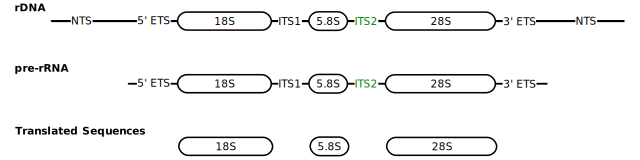
\includegraphics[width=\textwidth]{ITS_schematic.pdf}
    \caption[ITS2 structure overview]{Structure of Eukaryotic nuclear ribosomal DNA.
        rRNA genes exist in tandem repeats separated by nontranscribed spacers (NTS).
        These NTS are composed of internally transcribed spacers (ITS) and externally
        transcribed spacers (ETS).
        ITS2 is highlighted in green and forms an effective taxonomic barcode at sequence level 
        for eukaryotic species analyses.  The ITS2 secondary structure
        shows a greater level of conservation and can be used to investigate
        lower distance systematic relationships.  Figure was redrawn from \citep{Shi2005}}
\label{fig:its2_schematic}
\end{figure}

In many species the rDNA cistron is present in multiple copies
as tandem head-to-tail repeats varying in copy number from 1,2 copies
to thousands \citep{Torres-Machorro2010}.  While these copies are
frequently homogeneous there are many organisms that display
intranuclear variation \citep{Buchheim2011}.
For example, alveolates have been discovered with variant 
rDNA copies \citep{Stern2012,Galluzzi2004}. At 
different points in the life cycle of \textit{Plasmodium} spp. \citep{Nishimoto2008}
there is expression of SSU rRNA gene paralogues with up to 11\%
difference \citep{McCutchan1988,Chambouvet2015}.
Similarly, chlorophytes have previously displayed 
heterogeneity in rDNA copies \citep{Pillmann1997,Fama2000}.
Therefore, care must be taken not to assume intranuclear
homogeneity in phylogenetic analysis of ITS2 sequences \citep{Buchheim2011}


This said, ITS2 sequencing will identify the endosymbiont species in
the CCAP 1660/12, Yad1g1N and CCAP 1660/13 cultures. It will also offer a
method by which the clonality within the
photobiont populations can be investigated.  
By amplifying and sequencing a large number of 
ITS2 fragments from the same culture there is a reasonably
good chance that all the ITS2 level diversity will be sampled. 
If, on analysis, these sequences form multiple clades or 
display divergent groupings this could be strong evidence
for a multiple photobiont co-habitation within the \textit{P. bursaria}
host.  


Finally, one last means in which we sought to
gain additional insight into the host-endosymbiont
system was through the use of multiple-displacement amplification (MDA)
based sequencing \citep{Lasken2007}.  
Due to difficulties in obtaining sufficient
culture densities and the prevalence of putative sources of contamination
within the culture bulk genome sequencing was considered to be prone to 
major difficulties.  Therefore, MDA offered a way in which 
we could further investigate this question of photobiont clonality
while also generating a resource with potential use for further analysis.
For example, searching for potentially biologically significant genes
that are 
present in the genome but are not transcribed during endosymbiosis.
The utility of this genomic resource hinges on our ability to 
partition recovered genomes/contigs into the originating host
and endosymbiont genomes.  It is particularly important to do this
and effectively discard contaminant contigs derived from 
bacteria (food and symbionts) and viruses associated with the host. 



%However, this type of barcoding approach to species identification is 
%imperfect 
%
%It has been discovered that the rDNA-ITS2 sequence is uniform
%within each of the described groups of endosymbiont species/strains 
%\citep{(Hoshina et al. 2004, 2005; Gaponova et al. 2007; Summerer et al. 2008; Hoshina & Imamura 2008a; Luo et al. 2010).
%with up to 20\% differences in the ITS2 (despite very similar exonic SSU rRNA)
%Species concepts  - ITS2 vs 18S vs whatever \citep{Boenigk2012}
%Assembly of mini-metagenomes/sc genomes \citep{Nurk2013}

\subsection{Isolation of \textit{P. bursaria}}

One avenue that is important for an effective analysis of a host-endosymbiont
system is the ability to analyse the partners in isolation.  This can be used
to test individual hypotheses regarding each partner and  allows controlled
reintroduction experiments to be undertaken. 
Unfortunately,
the majority of extant, well-characterised endosymbioses display metabolic co-dependence
and therefore, host and endosymbiont cannot be isolated without one or other dying (i.e. they
form an obligate relationship as supposed to a facultative one). 

Fortunately, there have been numerous studies that have investigated the separation of 
host and symbiont in \textit{P. bursaria} - green algal systems e.g. \citep{Hosoya1995a,Achilles-Day2013,
Karakashian1963}. Most recently, the only transcriptomic analysis of this system by \citet{Kodama2014c}
investigated the differential global metatranscriptome profile of \textit{P. bursaria} Yad1g strain with 
 and without its \textit{Chlorella variabilis} 1N endosymbiont 
\citep{Kodama2014c}.   While, this is a different strain of both host and endosymbiont to the SW1-ZK 
strains in the CCAP1660/12 culture
(\textit{P. bursaria} and \textit{Micractinium reisseri}) reproduction of this endosymbiont
clearing offers a potential avenue by which to further investigate and, combined with RNAi 
to test the functional underpinning of this relationship. 

There have been several published methods
for clearing endosymbionts from host cells namely, the herbicide paraquat \citep{Hosoya1995a}, 
culturing under constant dark \citep{Karakashian1963}, herbicide DCMU \citep{Kodama2009a},
X-ray \citep{Wichterman1948}, and cycloheximide \citep{weis1984effect,Kodama2007}.
Therefore, we attempted three of these methods: specifically paraquat, cycloheximide, and 
constant darkness treatments with bacterial feeding 
in order to clear endosymbionts from the host \textit{Paramecium}.

\section{Aims}

In this chapter I will determine the exact algal endosymbiont strains present
in the principal \textit{Paramecium bursaria} cultures used throughout
this thesis and their relationships relative to one another and to
other green algae. 

I will also use this data and single cell genomics to investigate whether the algal
endosymbiont present in the \textit{Paramecium bursaria-Micractinium reisseri}
CCAP 1660/12 strains form a clonal population. 

Finally, I will discuss the attempts to remove the endosymbiont in the 
\textit{Paramecium bursaria} CCAP 1660/12 strain from the host.

\section{Methods}

\subsection{Taxonomic analysis}
    
\subsubsection{ITS2 sequencing}

\textit{Paramecium bursaria} CCAP 1660/12 and \textit{Paramecium bursaria} CCAP 
1660/13 cultures were maintained in New Cereal Life (NCL) media
at \SI{18}{\degreeCelsius} with 12:12 hour light/dark cycle.  In order to mitigate
the risk of sequencing free-living algae in the CCAP 1660/13 culture, ITS2
sequences were acquired from both pure culture samples and carefully purified samples.
Purification involved successive filtering and washing steps of isolated cells in sterile NCL media. 
Specifically, filtration using a \SI{10}{\micro\metre} filter, washing off, re suspension and 3 serial subcultures
in sterile NCL media. 

ITS2 sequences were amplified using 2 pairs of primers: ITS2-S2F primer (\(ATGCGATACTTGGTGTGAAT\))
binding to conserved 5.8S sequences from \citep{Chen2010} with the CHspeHLR1R \\
(\(CACTAGACTACAATTCGCCAGCC\))
reverse primer specific to chlorophyte 28S \citep{Hoshina2004} and the ITS4 primer \\
(\(TCCTCCGCTTATTGATATGC\))
\citep{white1990amplification} (see \cref{fig:its2_primers}).  The reason for the dual primer
approach was that it was observed in the smaller biological samples created during the cleaning
process that the ITS2-S2F - CHspeHLR1R primer pair wasn't amplifying ITS2 very efficiently
therefore the alternate primer pair was used. 

\begin{figure}
    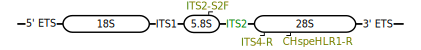
\includegraphics[width=\textwidth]{its2_primers.pdf}
    \caption[ITS2 primer locations]{Schematic diagram showing the location of the forward (ITS2-S2F) and reverse
    primers (CHspeHLR1R, ITS4-R) used for the amplification of ITS2 sequences in this study.
    CHspeHLR1R binds within the 28S whereas ITS4-R binds closer to the 5' end of the 28S.  Both
primer sets recover the full ITS2 sequence.}
    \label{fig:its2_primers}
\end{figure}

PCR conditions used were \SI{94}{\degreeCelsius} for \SI{5}{\minute} followed by
40 cycles of \SI{30}{\second} at \SI{94}{\degreeCelsius}, \SI{30}{\second} at \SI{56}{\degreeCelsius}
and \SI{45}{\second} at \SI{72}{\degreeCelsius}. This was followed by a final
elongation step of \SI{10}{\minute} at \SI{72}{\degreeCelsius}. 


PCR products were then cleaned up, cloned, sequenced
and processed using the same protocol as \citep{Maguire2014a}.
Briefly, the successfully amplified PCR products were gel-purified 
(Wizard SV Gel and PCR Clean-Up kit, Promega).
These products were then TA-cloned 
using Agilent's PCR StrataClone Cloning kit, blue-white screened and 5 clones
selected for each PCR product.  
Clones were then externally Sanger sequenced using the M13Rev primer
at MWG Eurofins. 
Flanking vector and primer sequences were removed, sequences trimmed to 
areas of high chromatograph quality and ambiguously defined bases corrected
using Sequencher \citep{Sequencher}.

From the 3 \textit{Paramecium bursaria} CCAP 1660/12 biological replicates
14, 9, and 11 ITS2 sequences were obtained respectively.
Similarly, from the 2 \textit{Paramecium bursaria} CCAP 1660/13 biological replicates
8 were obtained from sequences obtained from the culture directly, and 10
from the purified, washed samples (7 using ITS2-S2F-ITS4 primers and 3 using
ITS2-CHspe).  Additionally, 5 ITS2 sequences were acquired from the Yad1g1N
culture following the same protocol. 

In order to mitigate the risk of sequencing error masquerading
as true sequence divergence any sequences found in later phylogenetic
analysis to demonstrate single nucleotide changes from the consensus
of its clade placement was resequenced at MWG Eurofins in reverse 
using M13Uni.  Specifically, these were ITS-B18,
ITS-2, ITS-19, ITS-B6, ITS-B3, ITS-A7, ITS-6, ITS-B15,
ITS-10, ITS-9, ITS-15, and ITS-1.

See appendices (\cref{sec:app_its2}) for a full listing of trimmed sequences
and representative gel images of the cloning products.

\subsubsection{Phylogenetics}

ITS2 sequences used in \citep{Hoshina2010}, \citep{Hoshina2013} were retrieved
from genbank. 
The trimmed sequences and the established database sequences were then
aligned using MUSCLE \citep{Edgar2004}. This alignment was manually masked in the graphical 
SeaView \citep{Gouy2010} package.
jModelTest2 \citep{Guindon2003,Darriba2012} was then used to pick an appropriate substitution model.
Finally, phylogenies were inferred using the maximum likelihood
method via RAxML version 8 \citep{Stamatakis2014} with 1,000 bootstrap replicates.
Similarly, MrBayes \citep{Huelsenbeck2001} was used to infer the phylogeny using the bayesian
framework.  MrBayes used 2 independent runs of 4 Monte-Carlo Markov-Chains (MCMC) for
3,750,000 million generations (at which point the 2 runs were considered to have converged, 
as determined in Tracer v1.4 \citep{rambaut2007tracer}.  Trees were estimated
from the MCMC results with a burn-in of 250,000 generations.
Trees were then visualised and support values combined using TreeGraph2 \citep{Stover2010}.

Trees were rooted using a Microthamniales outgroup composed of
\textit{Trebouxia gigantea} AJ249577.2, \textit{Trebouxia arboricola} SAG219-1a Z68705.1,
\textit{Trebouxia jamesii} Hp-MT1 AJ511357.1, \textit{Trebouxia impressa} AJ249576.1,
\textit{Trebouxia corticola} AJ249566.1, and \textit{Trebouxia higginsiae} AJ249574.1.

\subsection{Single cell genomics}

\subsubsection{DNA extraction}

Individual \textit{P. bursaria} CCAP 1660/12 cells were removed from culture 
and washed three times in a successive series of 
\(10 \mu l\) drops of sterile modified 
New Cereal Leaf-Prescott (NCL) medium to minimise prokaryotic contamination from 
bacterial foodstocks in the culture media. 
Cells were added to a final \(10\mu l\) drop of sterile water before being added
to a microcentrifuge tube.

DNA was then extracted using a Cetrimonium bromide based method adapted from \citep{Winnepenninckx1993}. 
In brief,  \(748.5 \mu l\) of CTAB extraction buffer (at \(37\celsius\) and \(100 \mu l\) beads (Sigma, \(425 – 600 \mu m\); acid washed) 
were added and the tube was vortexed for 5 minutes. 
The tube was incubated for 50 minutes at \(37\celsius\), 
vortexed again for 5 minutes and incubated for 50 minutes at \(60\celsius\).  
This was to ensure lysis of the endosymbiont's chitinous cell wall.
DNA was extracted three times with phenol/chloroform/isoamylacohol (25:24:1, pH 8), washed with 70\% ethanol and 
re-suspended in \(2.5 \mu l\) TE (pH 8). 
Whole-genome amplification of purified genomic DNA was performed using the multiple-displacement amplification based
(MDA) Qiagen REPLI-g Single Cell Kit. 
The REPLI-g amplified gDNA was purified using a QIAamp DNA mini kit and eluted in \(100 \mu l\) elution buffer.

\subsubsection{Sequencing}

Five prepared libraries were put forward for sequencing 
(Pb-3, Pb-4, Pb-6, Pb-7 and Pb-8).   Samples were
multiplexed and were rapid sequenced in an Illumina
HiSeq 2500 in \SI{150}{\bp} paired-end mode. 

\subsubsection{Read pre-processing}

Trimmomatic \citep{Bolger2014a} was used to trim sequencing adapters (using sequences
provided by Exeter Sequencing Service) via the ILLUMINACLIP setting.
Reads were then quality trimmed at a minimum average SLIDINGWINDOW 
quality thresholds of Q5 and Q30. 

Q5 and Q30 trimmed reads were then error corrected using BayesHammer
\citep{Nikolenko2013} as built into the SPAdes assembler \citep{Bankevich2012}.

Trimmed and error corrected libraries were also then digitally normalised
\citep{Brown2012} to a coverage of 20 and with a \(k\)-mer size of 25.
Following this, \(k\)-mers were abundancy filtered \citep{Zhang2014,Zhang2015}
using the Khmer package \citep{Crusoe2015}.

\subsubsection{Assembly}

Assemblies were then generated using the following sets
of data:

\begin{itemize}
    \item Q5 trimmed reads with error correction
    \item Q30 trimmed reads with error correction
\end{itemize}

The following assemblers were used:
\begin{itemize}
    \item SPAdes assembler \citep{Bankevich2012,Nurk2013}
    \item SPAdes assembler with ``careful'' thresholding (runs MismatchCorrector and minimises the risk 
        of indels)
    \item MEGAHIT \citep{Li2015a}
    \item Platanus \citep{Kajitani2014}
%    \item SOAPdenovo2 \citep{Luo2012}
%    \item Hybrid \textit{De novo} Assembler (HyDA) \citep{Movahedi2014}
\end{itemize}

\subsubsection{Assembly assessment}

Assemblies were assessed and compared using the
QUality ASsessment Tool for genome assembly (QUAST) \citep{Gurevich2013a}
and key assembly metrics were compared (N50, N90, contig number
and length and total assembly size).


\subsubsection{Contig binning}
Contigs were subsequently cut into 10kb fragments for consistency
in binning and taxonomic assignment and obviate the difficulties
aligning very long sequences. 
Reads were then mapped back onto the final assembly using Bowtie2 
\citep{Langmead2012} 

Using the metagenomic binning tool, CONCOCT \citep{Alneberg2014}
contigs were binned into clusters based on sequence composition
and coverage features (derived from mapping data).
Coverage features were derived from a coverage and linkage table
generated via CONCOCT scripts built around BEDTools \citep{Quinlan2010,Quinlan2014}, Picard (\url{http://broadinstitute.github.io/picard/})
and Samtools \citep{Li2009} 
based parsing
of the bowtie2 alignment files.
Clustering was conducted using a Gaussian Mixture Model (GMM) \citep{Bishop2006}
and the number of clusters determined through variational Bayesian inference \citep{Corduneanu2001}.

All CONCOCT analyses were completed using a provided pre-configured 
Docker Image \citep{Merkel2014}, a form of lightweight 
distributable process isolation container.
This was downloaded from DockerHub (\url{https://hub.docker.com/r/binpro/concoct/})
on 2015-10-25.

Additionally, the cut contigs were taxonomically assigned 
using TAXAssign (\url{https://github.com/umerijaz/TAXAassign}) against the NCBI nt database. 
The BLAST database was downloaded using update\_blastdb.pl script (\url{http://www.ncbi.nlm.nih.gov/blast/docs/update_blastdb.pl})
and TAXAssign was run in parallel (using GNU parallel \citep{Tange2011a})
with a maximum of 10 reference matches
per contig a minimum percentage identity for assignment
to a given taxonomic level of 60, 70, 80, 95, 95, and 97
for Phylum, Class, Order, Family, Genus and Species respectively. 

CONCOCT clusters were then evaluated using the taxonomic assignments from TAXAssign
using the provided ``validate.pl'' script.

Finally, another attempt at taxonomic assignment using a custom ORF based pipeline was attempted:
\begin{itemize}
    \item ORFs with a minimum size of 300 were called using Tetrahymena and Universal encodings from contigs over \SI{500}{\bp} 
    \item ORFs were then clustered at 90\% identity using CD-HIT
    \item Diamond BLASTP searches were then done against the NR protein database
    \item Taxonomy was assigned to each contig based on the lowest common ancestor of all its
        ORFs with hits (via the ``lca\_mapper.sh'' accesory script in MEGAN)
    \item Contigs were then binned based on the identity of this taxonomic assignment:
        \begin{itemize}
            \item Endosymbiont contigs were all those assigned to Archaeplastida or a descendent node.
            \item Host contigs were all those assigned to Aveolata or a descendent node.
            \item Eukaryote was a super group containing all Eukaryote assigned contigs
            \item Contaminant contigs were all those assigned as Bacterial
            \item Viral contigs were all those assigned as Viral sequences. 
        \end{itemize}
\end{itemize}

\subsubsection{Variant calling}

A variant calling on the binned genomic contigs was attempted 
to assess the clonality of the endosymbiont. 
Briefly, the top 10 longest contigs binned as ``endosymbiont'' 
were retrieved and Q5 trimmed, error corrected reads aligned
to them using bowtie2 and output to BAM files for each library.
Library BAMs were then combined using samtools ``mpileup''
with a minimum mapQ threshold of 5.  All potential variants
with a mapping depth of 0 were filtered out.
SNPs were called from this filtered mpileup file
using a custom perl script designed for the 
the wheat genome project (pers. comms. Hall, Neil).
This SNP calling used a coverage cutoff of 10\%.

Called SNPs were then visualised and statistics
calculated using R.

\subsection{Endosymbiont elimination}

CCAP 1660/12 and Yad1g1N1 cultures in NCL media with were treated under the following
conditions to attempt to remove the endosymbiont. 
\textit{P. tetaurelia} were used as a control culture and was
given the same treatment. 

Paraquat was added at both \(1mg\mu l^{-1}\) and
\(0.5mg\mu l^{-1}\) concentrations.
Cultures were maintained under normal 12:12 lit:dark 
conditions at \(15\celsius\).  Cultures were inspected
daily using light microscopy and assessed for ``bleaching'' (i.e. loss of green 
appearance due to death of chlorophyll bearing alga). 

Cycloheximide was added to cultures at both \(1mg\mu l^{-1}\)
and \(10mg\mu l^{-1}\), again cultures were maintained under
standard 12:12 lit:dark condition and \(15\celsius\). 
Cultures when looking clear were subcultured and resuspended in 
NCL without cycloheximide.

Cultures were maintained in the dark without a lit phase
at \(15\celsius\) and inspected every 2 weeks for clearing.
This was to prevent providing too much light and 
further encouraging endosymbiont growth. 


\section{Results}

\subsection{ITS2 phylogeny}

The ITS2 phylogeny demonstrates a clear and well supported relationship in all samples 
between the CCAP 1660/12 and CCAP 1660/13 endosymbionts and the species described as 
\textit{M. reisseri} (see \cref{fig:its2_phylo}).  Additionally,
the Yad1g1N endosymbiont is positively identified as \textit{C. variabilis}. 
This phylogeny in general is consistent with previous ITS2 phylogenies \citep{Hoshina2010}.

\begin{figure}
    \centering
    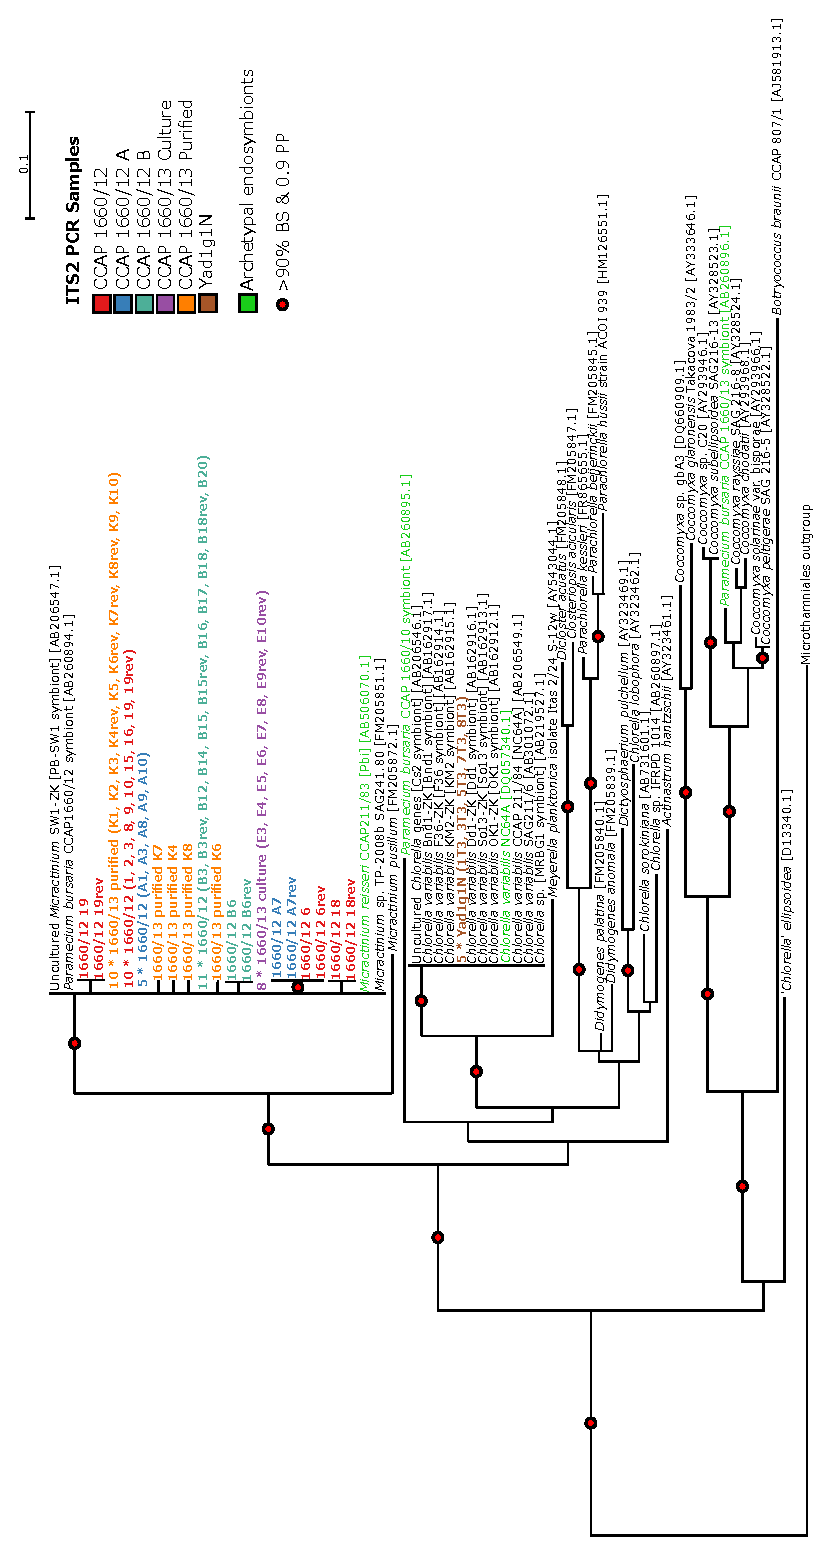
\includegraphics[height=0.8\textheight]{its_phylo.pdf}
    \caption[ITS2 phylogeny]{Combined MrBayes and RAxML phylogeny of all ITS2 sequences
    along with numerous reference ITS2 sequences from \citep{Hoshina2010,Hoshina2013}.
    This phylogeny highlights a single example of each of the 4 major groups of 
    \textit{P. bursaria} green algal endosymbionts i.e. \textit{Coccomyxa}, \textit{Micractinium reisseri},
    \textit{Chlorella vulgaris} and \textit{Chlorella variabilis}.  Multiple clones
    forming a polytomy have been collapsed into groups representing their biological
    replicate (i.e. 1660/12, 1660/12 A, 1660/12 B, 1660/13 Culture, 1660/13 Purified,
    and Yad1g1N). As can be observed all
    ITS2 sequences derived from CCAP 1660/12 replicates, and purified and non-purified CCAP 1660/13
    replicates form a single polytomy with established \textit{M. reisseri} sequences.  This indicates 
    that CCAP 1660/12 and CCAP 1660/13 endosymbionts are \textit{M. reisseri} and despite a few SNPs
form clonal populations.  Yad1g1N ITS2 sequences branch, as expected, with the other \textit{C. variabilis}
strains including NC64A.}
    \label{fig:its2_phylo}
\end{figure}

The ITS2 sequences of the CCAP 1660/12 culture demonstrated a 
variety of SNPs but never more than a single SNP difference from the basal \textit{M. reisseri}
polytomy.  These SNPs were grouped into 3 categories: 4 different SNPs that were not found in the
reverse complement and therefore represent likely sequencing error (1660-13-purified-K4, K8, K6 and K7),
3 different SNPs that were found in both forward and reverse sequencing (1660-12-B6, 1660-12-19 and 1660-12-18) and therefore
represent either true diversity or PCR error and finally 1 SNP that was found in 
forward and reverse sequencing and in two separate PCR reactions from different biological replicates (1660-12-A7 and 1660-12-6).
This featured a single base change from A to G (see \cref{fig:its2_snp}) at position 126 in the full masked alignment. 
This SNP could be the result of intranuclear variation of the ITS2 in the multicopy rDNA array.

\begin{figure}
    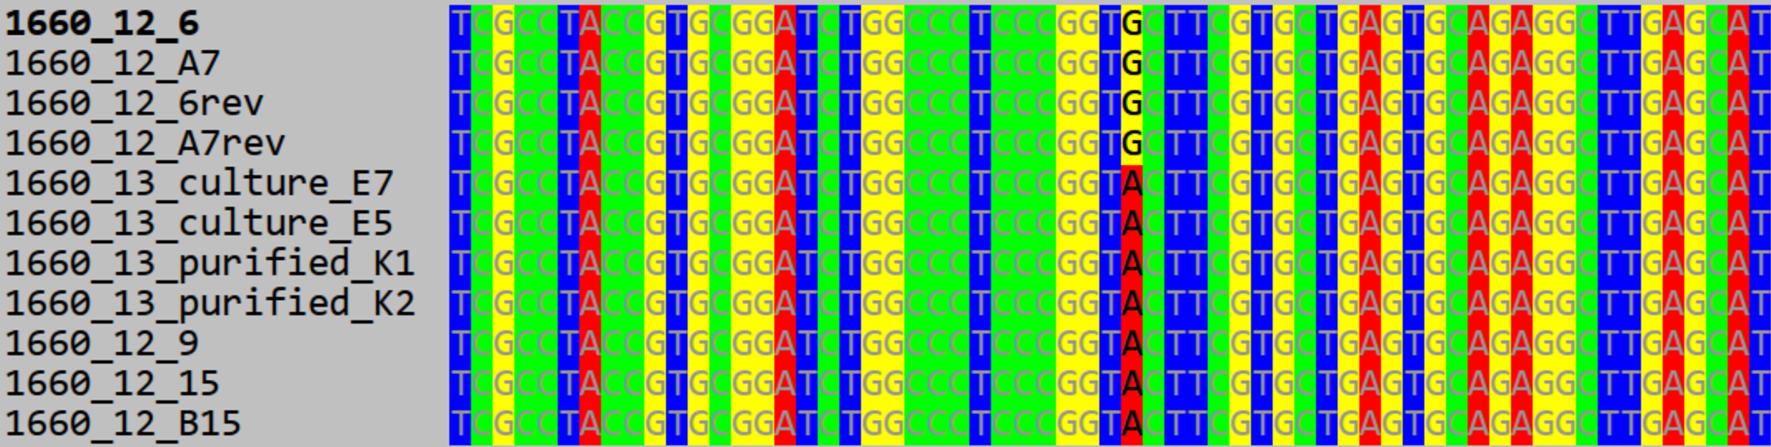
\includegraphics[width=\textwidth]{its_snp.pdf}
    \caption[ITS2 SNP alignment]{Alignment showing the sole SNP (at pos 126 in masked ITS2 alignment)
        that is likely to represent true diversity.  This indicates that the endosymbiont
    population is largely clonal with a small marginally divergent sub-population that has possibly
arisen during the endosymbiosis itself. Alternatively, this represents intranuclear variation of
the ITS2 across the genomic copies.}
    \label{fig:its2_snp}
\end{figure}

With the exception of these SNPs these sequences were identical to 3 from previously sequenced \textit{M. reisseri} endosymbionts, 
specifically CCAP 211/83 culture with \textit{P. bursaria} Pbi host (AB206547.1), the SW1-ZK symbiont from a \textit{P. bursaria} PB-SW1 host (AB506070.1),
and TP-2008b from the SAG241.80 culture (FM205851.1) (see \cref{fig:its2_phylo}).

This polytomy as the sister clade to other \textit{Micractinium pusillum} 
taxa was highly supported in both ML and Bayesian phylogenies (91.3\% of 
bootstraps and with a posterior probability of 1.00).
There was similarly high support for the separate branching of these sequences
from the clade containing the \textit{C. variabilis} and \textit{C. vulgaris} 
endosymbionts (\(87.3\%/1.00\)) and the existence of a clade comprising these 3
endosymbionts to the exclusion of any \textit{Coccomyxa} sequences was well supported
(\(89.3\%/0.95\)). 

Sequences from the Yad1g1N culture formed a clade with high support 
with other \textit{Chlorella variabilis} species including NC64A.
This support the identification of the endosymbiont in this culture
as \textit{C. variabilis} 1N.



\subsection{Single cell genomes}

\subsubsection{Sequencing and pre-processing}

The number of remaining reads in each library after trimming at a minimum average 
sliding window quality threshold of 30 and 5 can be found in \cref{tab:genome_trim}.

\begin{table}
    \centering
    \begin{tabular}{|c|c|c|c|}
        \hline
        \textbf{Sample} & \textbf{Raw PE Reads} & \textbf{Q30 Trimmed PE Reads} & \textbf{Q5 Trimmed PE Reads}\\
        \hline
        Pb-3 & \(3.523\cdot10^7\) & \(1.951\cdot10^7\) & \(2.737\cdot10^7\) \\
        Pb-4 & \(3.228\cdot10^7\) & \(2.606\cdot10^7\) & \(3.035\cdot10^7\) \\
        Pb-6 & \(3.291\cdot10^7\) & \(2.437\cdot10^7\) & \(2.962\cdot10^7\) \\
        Pb-7 & \(4.023\cdot10^7\) & \(2.642\cdot10^7\) & \(3.404\cdot10^7\) \\
        Pb-8 & \(3.869\cdot10^7\) & \(2.613\cdot10^7\) & \(3.246\cdot10^7\) \\
        \hline
    \end{tabular}
    \caption[The effect of read trimming threshold across libraries]{Summary of the number
    of surviving reads for Q5 and Q30 trims in each library}
    \label{tab:genome_trim}
\end{table}

After error correction the combined Q30 trimmed libraries comprised
\(1.218\cdot10^{8}\) paired end reads.  Similarly, the Q5 trimmed
libraries comprised \(1.538\cdot10^{8}\) reads. 

\subsubsection{Assembly}

Assemblies were compared using generated contigs and QUAST.
Assembly statistics were tabulated to allow comparison (\cref{tab:genome_ass_comparison}).
As we are interested in recapitulating as much genomic sequence as possible
from this complex metagenome but not necessarily to generate ``clean''
polished closed genome assemblies, the fact that the Q30-SPAdes assembly
generated both the longest total assembly (over twice the size of the nearest
assembly even when considering only contigs over \SI{1}{\kilo\bp}) as well
as the highest N50 and within \SI{2}{\kilo\bp} of the longest contig of all assemblies (generated
by Q5-SPAdes) was compelling. 

Generally, the SPAdes assemblers out-performed Platanus and MegaHit, likely due to 
being specifically designed for MDA based data.  Note, that all assemblies 
were completed with BayesHammer corrected reads so the difference in performance
cannot be attributed to this aspect of the assembly pipeline.

\begin{table}

    \resizebox{\textwidth}{!}{\begin{tabular}{|l*{5}{|r}|}
\hline
\textbf{Assembly} & textbf{Q30-MegaHit} & \textbf{Q30-Platanus} & \textbf{Q30-SPAdes-Careful} & \textbf{Q30-SPAdes} & \textbf{Q5-SPAdes} \\ \hline
        \# contigs ($\geq$ \SI{0}{\bp}) & 131,057 & {\bf 25,789} & 73,698 & 127,976 & 94,384 \\ 
        \# contigs ($\geq$ \SI{1000}{\bp}) & 14,960 & {\bf 486} & 13,301 & 21,808 & 12,614 \\ 
        Total length ($\geq$ \SI{0}{\bp}) & 73,350,696 & 6,289,036 & 73,691,706 & {\bf 142,281,712} & 81,478,234 \\ 
        Total length ($\geq$ \SI{1000}{\bp}) & 28,064,499 & 2,191,750 & 52,704,642 & {\bf 105,269,748} & 58,162,565 \\ 
\# contigs & 41,221 & {\bf 776} & 24,923 & 42,180 & 24,109 \\ 
Largest contig & 13847 & 78624 & 207156 & 207157 & {\bf 209,873} \\ 
Total length & 46,095,605 & 2,398,106 & 60,731,204 & {\bf 119,241,116} & 66,064,486 \\ 
GC (\%) & 38.81 & 33.68 & 37.78 & 37.85 & 39.27 \\ 
N50 & 1,246 & 6,386 & 4,949 & {\bf 7,163} & 6,334 \\ 
N75 & 769 & {\bf 2,875} & 1,845 & 2,277 & 2,188 \\ 
L50 & 10,444 & {\bf 112} & 2,937 & 3,530 & 2,241 \\ 
L75 & 22,405 & {\bf 249} & 7,974 & 11,103 & 6,716 \\ \hline
\end{tabular}}
\caption[Genome Assembly Statistics]{Assembly statistics generated by an analysis of contigs using QUAST. Best values are highlighted in bold.
    All statistics are based on contigs of size $\geq$ \SI{500}{\bp}, unless otherwise noted (e.g. "\# contigs ($\geq$ \SI{0}{\bp})" and "Total length ($\geq$ \SI{0}{\bp})" include all contigs).
N50 and N75 are the minimum contig length at which all contigs of that length are larger comprise 50\% and 75\% of the total assembly size. Similarly, L50 and L75 
are the number of contigs that are summed for a given N50 and N75 (i.e. lower is better). The highest values for
each metric across the assemblies is emphasised in bold.
This table shows that Q30 Platanus assembly generated the fewest and longest contigs overall, however the Q30-SPAdes assembly generated the longest
assembly by a considerable margin with the highest N50. 
}
\label{tab:genome_ass_comparison}
\end{table}

Plots of assembly GC (\cref{fig:assemb_gc}), cumulative length (\cref{fig:assemb_len})
further support Q30-SPAdes as both the longest assembly
but an assembly with similar GC profile to the other assemblies and contig length distribution.
Finally, the plot of X's indicates that Q30-SPAdes isn't a disproportionately highly gapped
assembly with low numbers of X's found in its longest contigs.  It should be noted, however,
that it does have a higher proportion of X's in shorter contigs than the other
assemblies (\cref{fig:assemb_nx}).

\begin{figure}
    \centering
    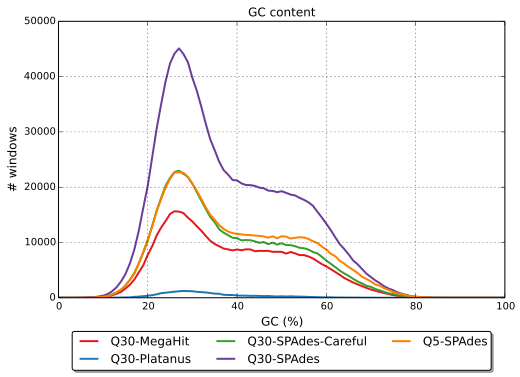
\includegraphics[width=0.8\textwidth]{assemb_gc.pdf}
    \caption[Genome assembly GC densities]{GC densities of the compared genome assemblies.  As expected
        all display a clear peak around \(30\%\) representing that the majority
    of the assemblies by length contigs are likely to be derived from the GC rich.
The height of the Q30-SPAdes peak reflects the relative size of this assembly.
Peaks around \(50\%\) GC may reflect endosymbiont contigs and possibly
bacterial contamination.}
    \label{fig:assemb_gc}
\end{figure}

\begin{figure}
    \centering
    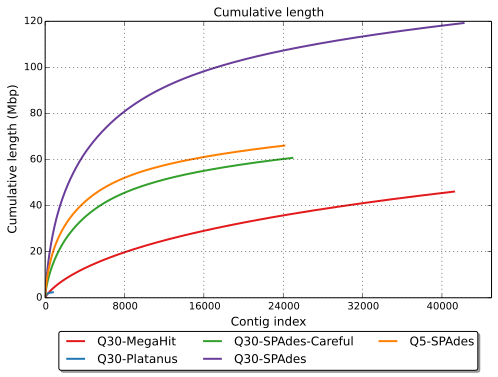
\includegraphics[width=0.8\textwidth]{assemb_cum_len.pdf}
    \caption[Genome Assembly Cumulative Contig Lengths]{The cumulative length of contigs as a function of
        contig number.  Again, this plot reflects
        that Q30-SPAdes generated the largest assembly
        by a considerable margin and while generating
        clean consistent contigs Platanus failed to recover
    many contigs found in other assemblies.}
    \label{fig:assemb_len}
\end{figure}

\begin{figure}
    \centering
    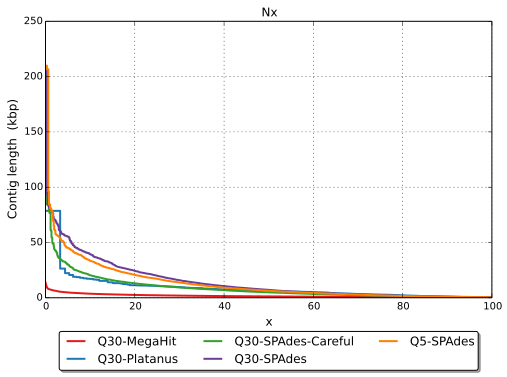
\includegraphics[width=0.8\textwidth]{assemb_nx.pdf}
    \caption[Genome assembly gaps]{The number of X (i.e. gap) in the assembled contigs as a function of their
        length.  This demonstrated that generally few Xs were assembled - however, it should 
        be noted that these are contigs and not assembly scaffolds and thus fewer Xs
    would be expected.}
    \label{fig:assemb_nx}
\end{figure}

Therefore, Q30-SPAdes assembly was selected for further analysis
and size filtered to exclude all contigs shorter than \SI{500}{\bp} 
to give 21,090 contigs. 

\subsubsection{Binning}

From the selected Q30-SPAdes assembly, the 21,090 contigs
were cut to 10kb fragments for decomposition to generate 64,852 contigs. 
18,277 of these 64,852 contigs were successfully given a
phylum level assignment, \cref{tab:genome_taxassign}.



\begin{table}
    \centering

\resizebox{\textwidth}{!}{\begin{tabular}{| r | r r c |}
\hline
\textbf{Source Group} & \textbf{Number of Contigs} & \textbf{Total Length} & \textbf{Phylum-Level Breakdown} \\
\hline
\textbf{Host} & 13 & 38,209 & Intramacronucleata\\
- & 2 & 140 & Apicomplexa\\
- & 1 & 163 & Colponemidia \\
\hline 
\textbf{Endosymbiont} & 12 & 2,758 & Chlorophyta\\
- &  12 & 3,987 & Streptophyta\\
- &  1 & 1,674  & Cyanobacteria\\
\hline
\textbf{Bacterial Contamination} & 16,230 & 13,435,718 & Proteobacteria \\
- & 468 & 669,751 & Firmicutes\\
- & 329 & 135,928 & Actinobacteria\\
- & 128 & 68,337 & Bacteroidetes/Chlorobi group\\
- & 1 & 241 & Deinococcus-Thermus\\
\hline
\textbf{Eukaryotic Contamination} & 605 & 640,915 & Ascomycota \\
- & 380 & 206,354 & Chordata\\
- & 74 & 38,529  & Arthropoda \\
- & 12 & 3,623 &  Basidiomycota\\
- & 7  & 2,150 & Nematoda \\
- & 1 & 61 & Platyhelminthes\\
- & 1 & 102 & Cnidaria\\
\hline
\textbf{Unknown} & 540 & 345,834 & Unclassified \\
\hline
\end{tabular}}
    \caption[Taxonomic Assignment of Genomic Contigs]{Summary of taxonomic assignments via TAXAassign grouped into putative ``source groups'' reflecting
		the most probable source of 10kb chunked contigs of that specific taxonomic provenance.  Of note, is the disproportionate
		number of contigs from contaminating sources. Specifically, bacteria such as Firmicutes and potential
    user contaminant in the form of Chordate assigned contigs.}
	\label{tab:genome_taxassign}
\end{table}

Contigs were clustered into 34 unique clusters by Concoct.
These taxonomic assignments were then used to validate the 34 contig clusters 
generated in Concoct (visualised in \cref{fig:concoct_clusters}) by considering them
as the ``ground-truth''.

\begin{figure}
	\includegraphics[width=\textwidth]{CONCOCT_clusters.pdf}
    \caption[Genomic contig clustering]{A low dimensional Principal Component representation of genomic contig
		cluster assignments.  Clusters are assigned via a Gaussian Mixture Model (GMM) 
		based on sequence compositional and coverage features as implemented in CONCOCT.
		Unfortunately, as can be observed clusters are both poorly distinguished even
        in the dimensions of the 2 principal components (PCA1 and PCA2) and there are many of them (34).
    This figure highlights how poorly resolved and noisy the decomposition of this single cell
    metagenome.}
	\label{fig:concoct_clusters}
\end{figure}

\begin{table}
    \resizebox{\textwidth}{!}{\begin{tabular}{| c || c | c |}
    	\hline
		 - & Positive & Negative \\
		 \hline
		 \hline
		True  &  Contigs with \textbf{same} taxonomic assignment   & Contigs with \textbf{different} taxonomic assignments \\
		& are assigned to the \textbf{same} cluster & are assigned to \textbf{different} clusters \\
		\hline
		False &  Contigs with \textbf{different} taxonomic assignments  & Contigs with the \textbf{same} taxonomic assignment \\
		& are assigned to the \textbf{same} cluster & are assigned to \textbf{different} clusters  \\
		\hline
    \end{tabular}}
    \caption[Explanation of Clustering Errors]{A contextual explanation of True and False Positive and Negatives in the context of contig binning/clustering.  Top left indicates what a
		True Positive (TP) means in this context, bottom left a False Positive (FP).  Similarly Top Right explains a True Negative (TN) and Bottom Right a
		False Negative (FN)}
	\label{tab:cluster_outcome_explanation}
\end{table}

Recall that Precision and Recall can be defined as follows:
\( Precision = \frac{TP}{TP+FP}\) and \(Recall = \frac{TP}{TP+FN} \)
where \(TP\) are True Positives and \(FP\) and \(FN\) are False Positives
and Negatives respectively (see \cref{tab:cluster_outcome_explanation} for an 
explanation of what these terms mean in the context of clustering).

CONCOCT assigned clusters were relatively precise \(0.912608\) 
therefore there were relatively few \(FP\) i.e. the majority of clusters 
contained contigs with the same taxonomic assignments. 

However, recall was relatively poor \(0.542250\) suggesting a
fair number of FN i.e. contigs with the same taxonomic assignments
were not confined to a single cluster and were spread over main clusters.

The \(F_1\)\footnote{\(F_1 = 2 * \frac{(precision * recall)}{(precision + recall)}\)} score for CONCOCT 
clustering was therefore \(0.680389\) under the assumption that 
TAXAssign represents the ground-truth. 

It is also worth noting that the 34 clusters had a relatively high level of mutual information
(Normalised Mutual Information of \(0.332022\) and a Rand Index of \(0.499741\)) suggesting
many small but highly similar clusters were created.  This level of similarity combined
with the poor recall suggests a greater number of clusters were inferred than was
present in the taxonomic assignment ground-truth.  This is likely due to
the variational inference of cluster numbers being partially reliant upon
sequencing coverage features.  As MDA is known to generate very uneven coverage 
due to amplification biases this likely explains the erroneous clustering.


Therefore, clustering and TAXAssign binning methods were abandoned and
the custom ORF based pipeline bins (\cref{tab:custom_tax_bin}) used
for variant calling.

\begin{table}
    \centering
    \begin{tabular}{|c|c|c|}
        \hline
        \textbf{Bin} & \textbf{Number of Contigs} & \textbf{Total Size (in \si{bp})} \\
        \hline
        Endosymbiont & 782 & 1,767,324\\
        Host & 3,451 &  24,294,611 \\
        \hline
        Other Eukaryotic & 1,646 & 7,237,238\\
        Bacterial and Unknown & 15,211 & 26,342,475 \\
        \hline
    \end{tabular}
    \caption[Custom Taxonomic Binning]{Results of the customised taxonomic binning,
    note the far less conservative binning compared with TAXAssign. Note this only
    consisted of contigs over \SI{500}{\bp} in length}.
\label{tab:custom_tax_bin}
\end{table}

\subsubsection{Variant Calling}

The variant calling demonstrated that the majority of potential
variants were present in almost all endosymbiont genomes (\cref{fig:var_contig}).
Indeed, the highest number of variants (\(\geq 75\)) were present in 
\(80-90\%\) of endosymbionts.

\begin{figure}
    \centering
    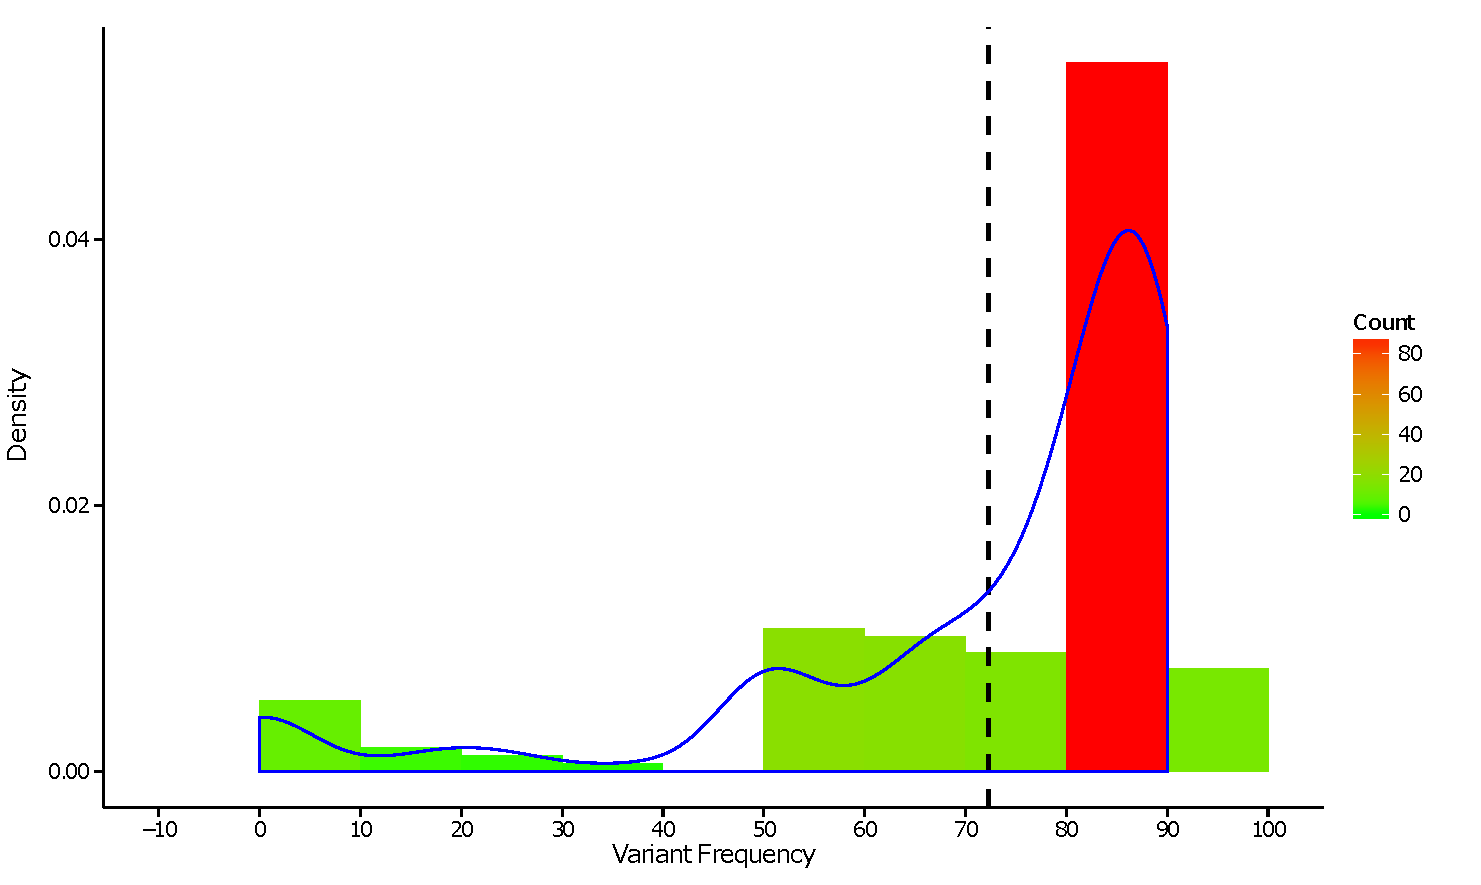
\includegraphics[width=\textwidth]{snp_variant_longest_contig.pdf}
    \caption[Endosymbiont variant count and frequency density]{
        Histogram summary of variant frequency in the longest 
        10 custom binned ``endosymbiont'' contigs (total length \SI{269,755}{\bp}).
        Variant frequency is the percentage of total chromosomes
        in the sample that share that variant and count axis shows
        the density (blue line).  The vertical dotted line indicates
        the mean of the sample and the heatmap shows absolute counts
        in the histogram bins. This figure shows the majority
        of variants are present in the majority of endosymbiont
    cells within the host.}
    \label{fig:var_contig}
\end{figure}

\subsection{Elimination of endosymbiont}

All elimination analyses focused on the \textit{P. bursaria}-\textit{M. reisseri}
CCAP 1660/12 strain.
After 1 week \(10\mu g ml^{-1}\) Paraquat treated CCAP 1660/12 were partially bleached
with few visible green \textit{M. reisseri} present in the cells under light
microscopy.
Unfortunately, after 2 weeks, and despite regular feeding, all CCAP 1660/12
treated with paraquat appeared to die with lysis of the \textit{Paramecium}.

To assess whether this phenotype was due to a too great concentration of paraquat
the experiment was repeated at a lower concentration  (\(1\mu g ml^{-1}\)).
Unfortunately, this led to the same process of gradual bleaching of the CCAP 
1660/12 cultures followed by their death. The difference being at the lower concentration
this occurred over a 6 week timeframe instead of 2 weeks.


A similar pattern was observed with both concentrations of
cycloheximide where \(10\mu g ml^{-1}\) treatment 
led to a reduction in endosymbiont abundance by 90\%
after 1 week followed promptly by host death. 
The lower concentration \(1\mu g ml^{-1}\) 
displayed the same pattern but over a 6 week period.

Finally, with subculturing and feeding cultures maintained in 
constant darkness did lead to gradual bleaching over 4-8 weeks.
However, after 10 weeks the cultures died with no visible
\textit{P. bursaria} cells.


\section{Discussion}

\subsection{CCAP 1660/12 and CCAP 1660/13 contain largely clonal \textit{M. reisseri} symbionts}

Phylogenetic analysis demonstrates that the endosymbiont present in the CCAP 1660/12
and CCAP 1660/13 is \textit{M. reisseri}.  The ITS2 sequences derived from these
two cultures across five different biological replicates (using both primer sets and with or without 
extra purification steps to minimise contamination from any algae present in the media) 
were all identical (with the exception of individual SNPs) 
to 3 separate previously published \textit{M. reisseri} ITS2 sequences. That this formed
a well supported clade with other \textit{Micractinium} sequences and was clearly a distinct
grouping from the other \textit{P. bursaria} endosymbiotic green algal species 
further supports the identity of the 1660/12 and 1660/13 endosymbionts as \textit{M. reisseri}.

While 8 different SNPs were identified in the ITS2 sequences, these never occurred in the same
sequence and half are easily attributable to sequencing error as they couldn't be recapitulated
in reverse sequencing of the same clone.  Of the remaining 4 SNPs that were validated
as not being sequencing error, only 1 was discovered in separate PCR reactions and biological replicates
and thus can putatively be attributed to genuine biological diversity and not merely PCR error
(ITS2-6 and ITS2-A7, A to G transition). Therefore, on the basis of ITS2 sequences
we cannot say the endosymbionts in CCAP 1660/12 and 1660/13 form a clonal population.
However, a single SNP in the hypervariable ITS2 region represent very recent and minor
divergence.  The most likely explanation is that this represents the emergence of a slightly modified
line of endosymbionts within the clonal endosymbiont population of the CCAP 1660/12 culture or intranuclear
variation within a single clonal population.  The distribution of SNP variants on endosymbiont binned
contigs supports this hypothesis. This is because the majority of SNPs were detected to be 
present in \(73\%\) or more of endosymbiont chromosomes. 
Due to the uniformity of the ITS2 sequences there is no evidence of multi-strain photobiont co-habitation as 
described by \citep{Hoshina2012}.

It should be noted that the majority of ITS2 based studies make use of the secondary structure (predicted
using tools such as RNAstructure \citep{Mathews2004}) in inference \citep{Schultz2009}. 
This increases reliability of phylogenetic inference \citep{Keller2008} allows ITS2 to be used
to distinguish higher taxonomic levels \citep{Coleman2003}, and plays a role
in resolving the thorny problem of species determination \citep{Muller2007}. 
However, as the endosymbiont species ITS2 secondary structures have already been extensively
investigated (e.g. \citep{Hoshina2008,Hoshina2010}) and are generally better suited
for analysis of more divergent taxa, it was considered 
unecessary to conduct structural analysis for taxonomic analysis of these
endosymbionts.

\subsection{Reliability of culture collection}

One clear result and point worth raising is that contrary to previous studies 
(accession \(AB260896.1\) \citep{Hoshina2008}) and CCAPs culture description 
CCAP 1660/13 does not contain a \textit{Coccomyxa} endosymbiont and contains 
an identical \textit{M. reisseri} endosymbiont to the CCAP 1660/12 culture. 
Unfortunately, on communication with CCAP it emerged that 
the 1660/12 strains in their collection are no longer available
and that CCAP 1660/13 had apparently become overgrown by free-living \textit{Coccomyxa}. 
Therefore it is likely that the previous finding of \textit{Coccomyxa} ``endosymbionts'' in
CCAP 1660/13 \citep{Hoshina2008} represents accidental contamination and sequencing 
of the free-living \textit{Coccomyxa} also present in the culture. 

The identical nature of the CCAP 1660/12 and CCAP 1660/13 endosymbioses is perhaps not surprising
when it is emphasised that these cultures were isolated from the same
pond (Cambridge, UK) by CCAP. 

This demonstrates the necessity of not taking culture collection labels and taxonomic
assignments on faith. It is critical to thoroughly determine that all received
cultures actually contain the organism.

\subsection{MDA metagenomes are non-trivial}

The biases induced by MDA in single cell genomes are known to be 
formation of chimeric sequences and the amplification
of undesired contaminant sequences \citep{Binga2008}.
Additionally, despite a theoretical basis that
the amplification coverage bias should be random \citep{Hosono2003}
there is evidence disputing this in practice \citep{Ellegaard2013}.
The magnitude of this bias is related to the starting
quantity of DNA \citep{Ellegaard2013a}.
Fortunately, there does not appear to be any bias
related to GC \citep{Ellegaard2013a}.
An increase in the number of starting cells to the range of
a few hundred to a few thousand cells
has been observed to improve amplification considerably \citep{Ellegaard2013a}. 
Unfortunately, increasing the number of cells in the case
of CCAP 1660/12 \textit{P. bursaria} - \textit{M. reisseri} system
would likely compound issue with bacterial contamination due 
to both a greater sample volume leading to greater inclusion
of food bacteria living in the media and an increase in the
number of partially digested bacterial (and viral) symbionts
associated with the host. 

SPAdes, by far, generates the best assemblies of complex
MDA-based metagenomes of the assembly tools trialled. 
This cannot be attributed to the effective read error correction
implemented as part of SPAdes via BayesHammer as all assemblies
were completed on BayesHammer error corrected reads. The performance
of SPAdes is likely attributable to two factors: it is specifically
designed to handle MDA-based single cell assemblies and thus is 
highly tolerant of the coverage variability observed and secondly
it is the lone genome assembler that effectively utilised
paired-end data during assembly.  The vast majority of assemblers
will only utilise this data in ad-hoc post-assembly heuristic operations
to improve contigs and scaffold the dataset.  On the other hand,
SPAdes generates the assembly de-Bruijn using siamese rectangular
graphs that incorporate both forward and reverse reads and their 
respective insert. 
In future, it may be worth re-analysing this data using
other MDA-specific tools such as HyDA to assess their performance. 

The relative performance of Q30-SPAdes with and without the ``careful''
setting is interesting. This setting minimises the risk of mismatch and indels
found in the assembly.  This led to assembly with statistics relatively similar
to that of the Q5-SPAdes assembly.   However, on correspondence with the developers
of SPAdes it emerged that there was a bug in this setting in the version
of the assembler used within this study leading it to be highly conservative
and discard many assembled contigs that were unlikely to be mismatches. 


Finally, the poor performance of CONCOCT suggests that coverage and composition
are not effective metrics by which to decompose an MDA-based metagenome
into constituent ``bins''.  The poor recall and high similarity indices between
the clusters suggests that a greater number of clusters were inferred than was present
in the ground truth of the taxonomic assignments.  This likely represents the effect of
biased amplification in MDA (therefore heterogeneous variable coverage) on
the variational inference of the number of clusters and the utility of the coverage 
feature in general.  This means, therefore, in MDA-based metagenomes standard metagenomic
binning pipelines that are reliant on coverage metrics (even partially as in the case
of CONCOCT) are not effective. 

This problem is somewhat symptomatic of the current state of the tool ecosystem
for MDA-based eukaryotic metagenomes. The few MDA-orientated analysis
tools focus on the assembly of bacterial systems whereas the majority of the metagenomic
tools are based on features and metrics such as coverage that are only
consistent in conventional non-MDA bulk genomic studies. 
Ideally, future research will improve the ease of analysis and assembly
of datasets such as this.

\subsection{Metabolic co-dependence in the CCAP 1660/12 system}

Due to the repeated failure to create endosymbiont free \textit{Paramecium}
hosts from the CCAP 1660/12 cultures using 3 of the major accepted
methodologies (cultivation in darkness \citep{Karakashian1963},
paraquat \citep{Hosoya1995a,Tanaka2002} or cycloheximide \citep{weis1984effect})
we are forced to address the possibility that the \textit{Micractinium reisseri}
endosymbiont and \textit{P. bursaria} system in CCAP 1660/12 and CCAP 1660/13
cultures forms an obligate system.  By some unidentified mechanism, metabolic
co-dependence may have become fixed in this culture. 

Cycloheximide does partially inhibit host protein synthesis
\citep{weis1984effect,Kodama2007,Kodama2008,Kodama2009a}
therefore it is possible that in the host strain found in the
CCAP 1660/12 culture that this partial inhibition is lethal to both
host and endosymbiont. However, the failure of this method in conjunction
with the Paraquat, a herbicide which theoretically should only affect the endosymbiont, 
and constant dark culturing suggests it is potentially the loss of the endosymbiont
that is lethal to the host cells (as adequate bacterial
foodstocks were included in these cultures).   

The one major method that wasn't attempted was the use of 3-(3,4-dichlorophenyl)-1,1-dimethlyura (DCMU)
an established blocker of photosystem II \citep{VanGorkom1974}. 
However, DCMU has previously been found to be mildly toxic in \textit{P. bursaria}, 
affecting the sexual reproduction system \citep{Miwa2009} therefore, this would
have proven unlikely to show different results in either the case of a particularly 
``sickly'' host strain or obligate endosymbiosis. 


This result indicates the presence of key differences between the current state of this
endosymbiosis and the previously studied \textit{C. variabilis} endosymbiosis
studied by \citep{Kodama2014c}.  Therefore, a comparative analysis of these systems
could theoretically shed light on the mechanism by which metabolic co-dependence
has become fixed in one system. Alternatively, this difference may just reflect the nature of two
different, independently acquired endosymbioses with different species and strains
of both host and endosymbiont. 


Another avenue of study that we did not investigate was that of
isolation of endosymbiont into free-living cultures \citep{Achilles-Day2013a}. This would allow
us to establish whether green algae such as \textit{Micractinium} that have obligate
hosts are themselves obligate endosymbionts.  There is some evidence pointing
towards this in nature, with the widespread predation of \textit{M. reisseri}
and \textit{C. variabilis} by their specific PBCV virotypes as well as the relative
paucity of natural free-living strains of these species.  To my knowledge, there
has only been a single isolated and characterised free-living \textit{M. reisseri} \citep{Abou-Shanab2014}
example and no \textit{C. variabilis} examples.  However,
this said, algae have previously been isolated from the CCAP 1660/13 culture \citep{Achilles-Day2013a}.
We have demonstrated via ITS2 sequencing that the endosymbionts in CCAP 1660/13 are the same
as those in CCAP 1660/12. Therefore, if these isolated algae are actually endosymbionts (as supposed
to the free-living \textit{Coccomyxa} sp. that overgrew the culture shortly after this study
was published) then the \textit{M. reisseri} endosymbiont is capable of living without
the host and is not an obligate endosymbiont despite \textit{P. bursaria} being an obligate host.  

\section{Conclusions}

Therefore, on the basis of ITS2 sequencing the CCAP 1660/12 culture endosymbiont is
a strain of \textit{Micractinium reisseri}.  Additionally, the CCAP 1660/13
endosymbiont has been misclassified as a strain \textit{Coccomyxa} and
is the same \textit{Micractinium reisseri} species found in the CCAP 1660/12 
culture. I have confirmed the Yad1g1N endosymbiont as being \textit{C. variabilis}
1N.  Despite poor performance in genome assembly, the evidence of
the genomes and ITS2 data seem to indicate that this endosymbiont
forms a clonal or near clonal population within the CCAP 1660/12
endosymbiont.  Similarly, on the basis of ITS2 diversity the Yad1g1N culture
contains a clonal 1N endosymbiont population.
At a minimum, a single strain of \textit{M. reisseri} 
comprises the sole green algal endosymbiont in the CCAP 1660/12
and 1660/13 cultures although there may be intranuclear variation of the ITS2
or it may be actively evolving as evidenced
by a small divergent sub-population.

Finally, the \textit{Micractinium reisseri} endosymbiont in cultures CCAP 1660/12 
CCAP 1660/13 has potentially become metabolically co-dependent with the host.
The host appears incapable of survival without the endosymbiont, therefore,
it is important to attempt to identify the differences between the demonstrably
facultative relationship between the Japanese Yad1g1N strains (used in \citep{Kodama2014c}) 
and the putatively obligate CCAP 1660/12. Identifying these differences may pinpoint
the mechanism by which metabolic co-dependence becomes fixed in \textit{P. bursaria}
- green algal endosymbioses.
